\documentclass[12pt,a4paper,final]{article}
\usepackage[utf8]{inputenc}
\usepackage[english]{babel}
\usepackage{amsmath}
\usepackage{amsfonts}
\usepackage{amssymb}
\usepackage{graphicx}
\usepackage[left=3cm,right=2.5cm,top=2.5cm,bottom=2.5cm]{geometry}
\author{Diogo Silva}
\begin{document}
\section{Datasets}
2 different Gaussian mixtures of 1800 points were used, with dimensions 2 (Fig. \ref{fig:mix}) and 6 respectively.

\begin{figure}[hbtp]

\centering
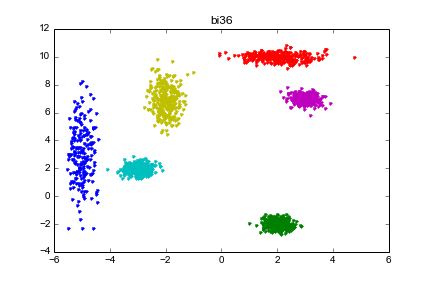
\includegraphics[scale=0.8]{figure.png}
\caption{Gaussian mixture with 2 dimensions.}
\label{fig:mix}
\end{figure}

\section{Tests}
Regarding the Quantum K-Means (QK-Means), the tests were performed using 10 oracles, a qubit string length of 8 and 100 generations per round. The \textit{classical} K-Means was executed using the \textit{k-means++} centroid initialization method. Since QK-Means executes a classical K-Means for each oracle each generation, the number of initializations for K-Means was $\#oracles \times \#generations \times factor$, where $factor$ is a adjustable multiplier. Each test had 20 rounds.

All tests were done with 6 clusters (natural number of clusters). Two tests were done with the two dimensional dataset: one with a $factor=1.10$ (increase initializations by 10\%) and another with $factor=1$. I'll call these tests T1 and T2. The test done with the six dimensional dataset (T3) used $factor=1.10$.

\section{Results}
\subsection{Timing results}

\begin{table}[h]
\caption{Timing results for the different algorithms in the different tests. Fitness time refers to the time that took to compute the DB index of each solution of classical K-Means. All time values are the average over 20 rounds and are displayed in seconds.}
\label{my-label}
\begin{tabular}{l|l|l|l|l|l|}
\hline
\multicolumn{1}{|l|}{Dataset}        & Algorithm         & Mean        & Variance    & Best      & Worst     \\ \hline
\multicolumn{1}{|l|}{T1}             & QK-Means          & 62.02642975 & 0.077065212 & 61.620424 & 62.579969 \\ \hline
\multicolumn{1}{|l|}{bi36}           & K-Means           & 6.4774672   & 0.002501651 & 6.352554  & 6.585451  \\ \hline
                                     & K-Means + fitness & 70.2238286  & 0.022223755 & 69.889105 & 70.548572 \\ \cline{2-6} 
                                     & fitness           & 63.7463614  & 0.019722105 & 63.536551 & 63.963121 \\ \hline
\multicolumn{1}{|l|}{T2}             & QK-Means          & 64.22347165 & 0.056559152 & 63.807367 & 64.807373 \\ \hline
\multicolumn{1}{|l|}{bi36\_noFactor} & K-Means           & 5.71167475  & 0.004903253 & 5.581391  & 5.877091  \\ \hline
                                     & K-Means + fitness & 62.7021533  & 0.066919692 & 62.180021 & 63.417207 \\ \cline{2-6} 
                                     & fitness           & 56.99047855 & 0.062016439 & 56.59863  & 57.540116 \\ \hline
\multicolumn{1}{|l|}{T3}             & QK-Means          & 74.4917966  & 0.067688312 & 74.12105  & 74.976446 \\ \hline
\multicolumn{1}{|l|}{sex36}          & K-Means           & 8.291648    & 0.007015777 & 8.160859  & 8.426203  \\ \hline
                                     & K-Means + fitness & 72.36315915 & 0.05727269  & 71.856457 & 73.031841 \\ \cline{2-6} 
                                     & fitness           & 64.07151115 & 0.050256913 & 63.695598 & 64.605638 \\ \cline{2-6} 
\end{tabular}
\end{table}

The mean computation time of classical K-Means is an order of magnitude lower than that of QK-Means. However, in classical K-Means the solution typically chosen if the one with lowest sum of euclidean distances of points to their attributed centroid. To make a fair comparisson between the two algorithms, the Davies-Bouldin index of all classical K-Means solutions was computed and used as the criterea to choose the best solution. When this is done, we can see that the total time of classical K-Means is actually higher that that of QK-Means in T1 and T3, but this is only due to the 1.10 multiplier on the number of initializations. In T2, possibly the fairest comparisson, the computation times become very similar with only a 2\% difference between the two algorithms.

\subsection{Accuracy results}

\subsubsection{Comparison}
\begin{table}[h]
\caption{All values displayed are the average over 20 rounds, except for the Overall best which shows the best result in any round. The values represent the Davies-Bouldin fitness index (low is better).}
\label{my-label}
\begin{tabular}{l|l|l|l|l|l|l|}
\hline
\multicolumn{1}{|l|}{Dataset} & Algorithm & Best        & Worst       & Mean        & Variance    & Overall best \\ \hline
\multicolumn{1}{|l|}{T1}      & QK-Means  & 15.42531927 & 32.29577426 & 19.94704511 & 21.23544567 & 15.42531927  \\ \hline
                              & K-Means   & 15.42531927 & 25.44913817 & 16.25013365 & 1.216919278 & 15.42531927  \\ \hline
\multicolumn{1}{|l|}{T3}      & QK-Means  & 22.72836641 & 65.19984617 & 36.10699242 & 78.14043743 & 22.71934191  \\ \hline
                              & K-Means   & 22.71934191 & 46.72231967 & 26.18440481 & 22.96730826 & 22.71934191  \\ \cline{2-7} 
\end{tabular}
\end{table}

The most relevant result in the table above is the mean of the best index. The value is the average over all rounds of the best solution in each round and it provides insight on the average performance of the algorithm. The results suggest that both algorithms perform equally well. The best overall result of each algorithm in all rounds is exactly the same. In T3, the mean performance of classical K-Means is marginally better.

I speculate that if classical K-Means was using only the sum of euclidean distances and not the DB index, the average performance would be worse. As it stands, choosing to use DB index with classical K-Means possibly represents a tradeoff between speed and accuracy.

\subsubsection{QK-Means}

Here we'll analyse a bit what's happening within each QK-Means execution. One would expect for the population's fitness variance to decrease over the generations, as the probabilities for previous known solutions increase. The convergence of the population mean would also be expected to decrease for the same reason. However, experimental (Fig. \ref{fig:mean_evo} and \ref{fig:var_evo}) results don't suggest any of these expectations (the results of T1 and T3 suggest the same). This may be due to low number of generations or simply because the random generation of initial centroids isn't influenced enough by the qubit probabilities.

\begin{figure}[hbtp]
\centering
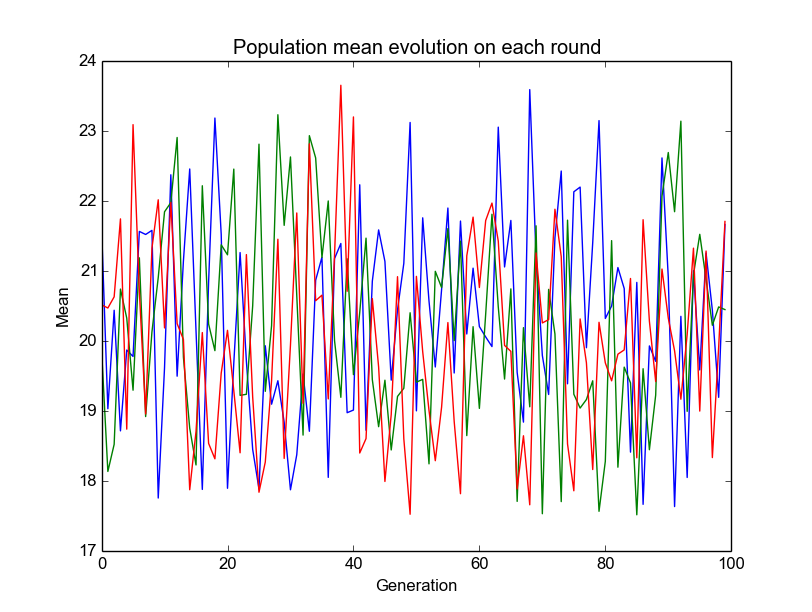
\includegraphics[scale=0.6]{bi_nofactor_mean.png}
\caption{DB index mean of the population in T2. Only 4 rounds represented.}
\label{fig:mean_evo}
\end{figure}

\begin{figure}[hbtp]
\centering
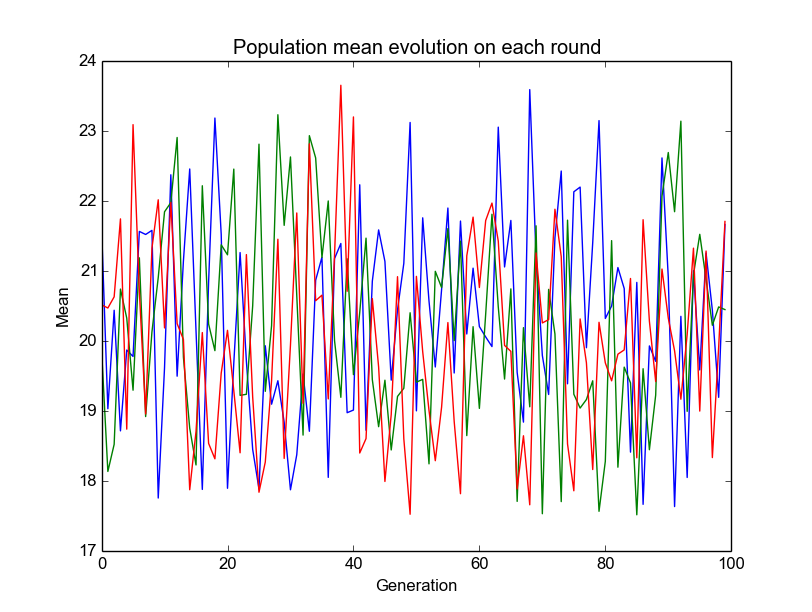
\includegraphics[scale=0.6]{bi_nofactor_mean.png}
\caption{DB index variance of the population in T2. Only 4 rounds represented.}
\label{fig:var_evo}
\end{figure}

Analyzing the evolution of the DB index of the best solution over the generations (Fig. \ref{fig:best_evo} and \ref{fig:best6_evo}) gives some insight on the rate of convergence. In both tests it's clear that the best solution is often reached in a quarter of the total generations. More detail can be seen in the following table.

\begin{table}[h]
\caption{The values represent generations.}
\label{my-label}
\begin{tabular}{|l|l|l|l|l|}
\hline
	 & Mean & Variance & Best     & Worst     \\ \hline
T1   & 17.25    & 70.2875  & 3     & 33 \\ \hline
T3   & 28.05    & 568.6475 & 2     & 90 \\ \hline
\end{tabular}
\end{table}


\begin{figure}[hbtp]
\centering
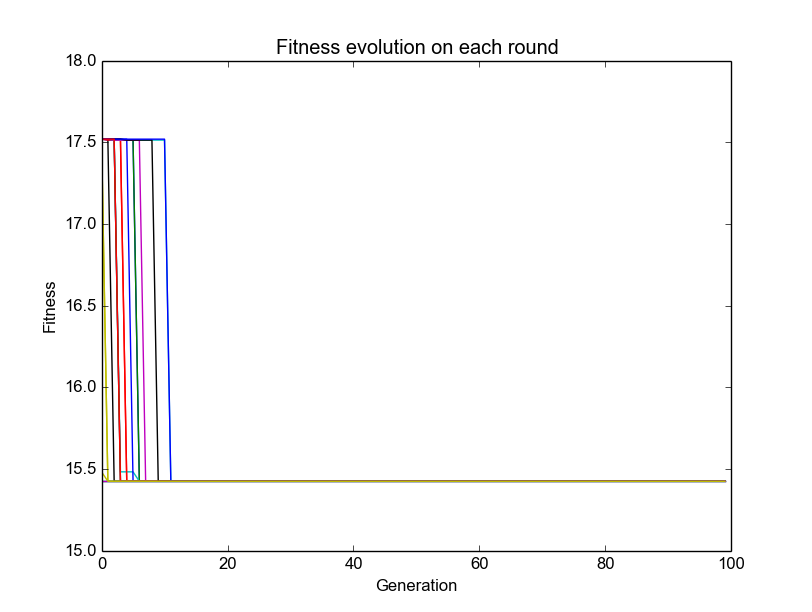
\includegraphics[scale=0.6]{bi_nofactor_evo.png}
\caption{DB index of best solution in T2.}
\label{fig:best_evo}
\end{figure}

\begin{figure}[hbtp]
\centering
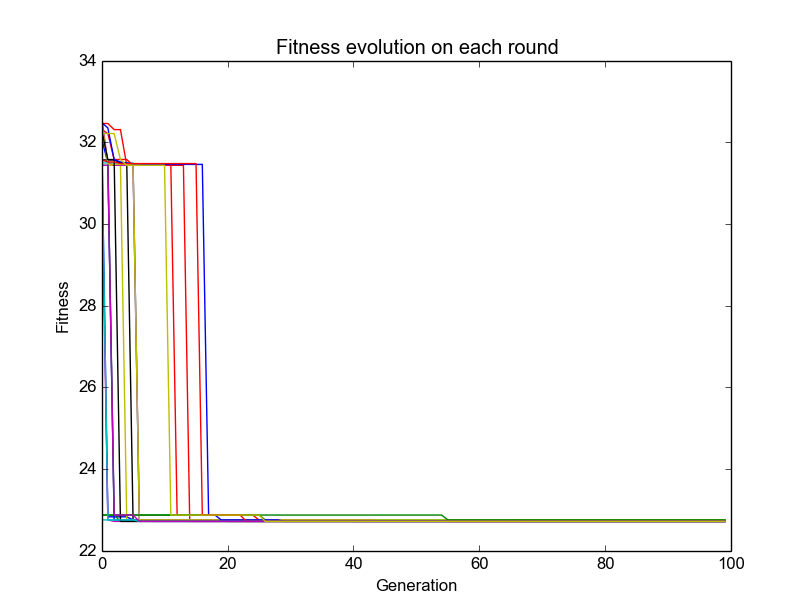
\includegraphics[scale=0.6]{sex_evo.png}
\caption{DB index of best solution in T3.}
\label{fig:best6_evo}
\end{figure}

\end{document}